%\documentclass[dvips,red]{beamer}
%\documentclass[red,xcolor=dvipsnames]{beamer}
\documentclass[xcolor=dvipsnames]{beamer}
\usepackage[utf8]{inputenc}
\usepackage{etex}
\usepackage[T1]{fontenc}
\usepackage[english,german]{babel}
\usepackage{amsmath,amsfonts,amssymb}
%\usepackage{dsfont}
\usepackage{hyperref}
%\usepackage{colortbl}
%\usepackage{rotating}
\usepackage{textcomp}
\usepackage{amsbsy}
\usepackage{marvosym} % Blitz
\usepackage{multicol}
\usepackage{helvet}
\usepackage{xcolor}
\usepackage{graphicx}
\usepackage{braket}
\usepackage{units}
\usepackage{multirow}
%\usepackage{overcite}
%\usepackage{bibgerm}
%\usepackage{inlinebib}
%\usepackage[absolute,overlay]{textpos}
\usepackage{booktabs}
\usepackage{appendixnumberbeamer}
\usepackage{animate}

\usepackage{tikz,pgfplots}
\usetikzlibrary{positioning,fadings,patterns,decorations}

   \tikzfading[name=fade inside,
            inner color=transparent!90,
            outer color=transparent!40]
   \tikzfading[name=fade out,
            inner color=transparent!0,
            outer color=transparent!90]

\pgfdeclaredecoration{stars}{initial}{\state{initial}[width=6pt,next state=star1]
{}
\state{star1}[width=4pt,next state=gap]{\pgfuseplotmark{star}}
\state{gap}[width=4pt,next state=star1]{}
\state{final}{\pgfpathmoveto{\pgfpointdecoratedpathlast}}
}

\pgfdeclaredecoration{starstars}{initial}{\state{initial}[width=6pt,next state=star1]
{}
\state{star1}[width=4pt,next state=star2]{\pgfuseplotmark{star}}
\state{star2}[width=4pt,next state=gap]{\pgfuseplotmark{star}}
\state{gap}[width=4pt,next state=star1]{}
\state{final}{\pgfpathmoveto{\pgfpointdecoratedpathlast}}
}
\tikzset{
dashStar/.style={dash pattern=on 4pt off 4pt,postaction={decorate,decoration=stars}},
dashStarStar/.style={dash pattern=on 4pt off 8pt,postaction={decorate,decoration=starstars}},
}

\definecolor{diplom1}{rgb}{0.0 0.4 1.0}
\definecolor{diplom2}{rgb}{0.0 0.0 0.6}
\definecolor{diplom3}{RGB}{153,0,0} %unirot
\definecolor{diplom4}{RGB}{232,215,23} 
\definecolor{diplom5}{RGB}{51,37,60} 
\definecolor{AUbluedark}{RGB}{0,37,70} 
\definecolor{AUbluelight}{RGB}{0,61,115} 

%\definecolor{diplom1}{rgb}{0,0.75,0.75}
%\definecolor{diplom2}{RGB}{153,0,0}

%\newrgbcolor{diplom1}{0.3 0.6 1.0}
%\newrgbcolor{diplom2}{0.8 0.1 0.7}

%\usetheme{CambridgeUS}
%\usetheme{Madrid}
\usetheme{Pittsburgh}
%\usecolortheme{mycrane}
%\usecolortheme{orchid}
%\usecolortheme{dove}
%\setbeamercolor{background canvas}{bg=black}
%\setbeamercolor{normal text}{fg=white,bg=black}
%\setbeamercolor{title}{fg=white,bg=black}
%\setbeamercolor{frametitle}{fg=white,bg=black}
%\usebeamercolor[fg]{normal text}
\usecolortheme[named=AUbluelight]{structure}
%\setbeamercolor*{block body}{bg= white}
%\setbeamercolor*{block title}{bg= diplom2}

%\setbeamercolor{itemize item}{fg=white}
%\setbeamercolor{itemize subitem}{fg=white}
%\setbeamercolor{itemize subsubitem}{fg=white}

\setbeamercovered{transparent}

\beamertemplatenavigationsymbolsempty


%Finde die Bilder
\graphicspath{{bilder/}}

\setcounter{tocdepth}{1}
\newcommand{\nocontentsline}[3]{}
\newcommand{\tocless}[2]{\bgroup\let\addcontentsline=\nocontentsline#1{#2}\egroup}
\DeclareMathOperator\erfc{erfc}

\begin{document}
 

\title[]
{Collaborating using git}
\subtitle{Branches}
\author[E. Fasshauer]{Elke Fasshauer}
\institute[]{University of Tübingen}
\date[2.11.21]{2nd November 2021}

%\titlegraphic{\includegraphics[scale=0.15]{pumuckl_jonglage.pdf}}

% Title page
\begin{frame}
\titlepage
\end{frame}

\begin{frame}{Where to go for the exercise}

\begin{center}
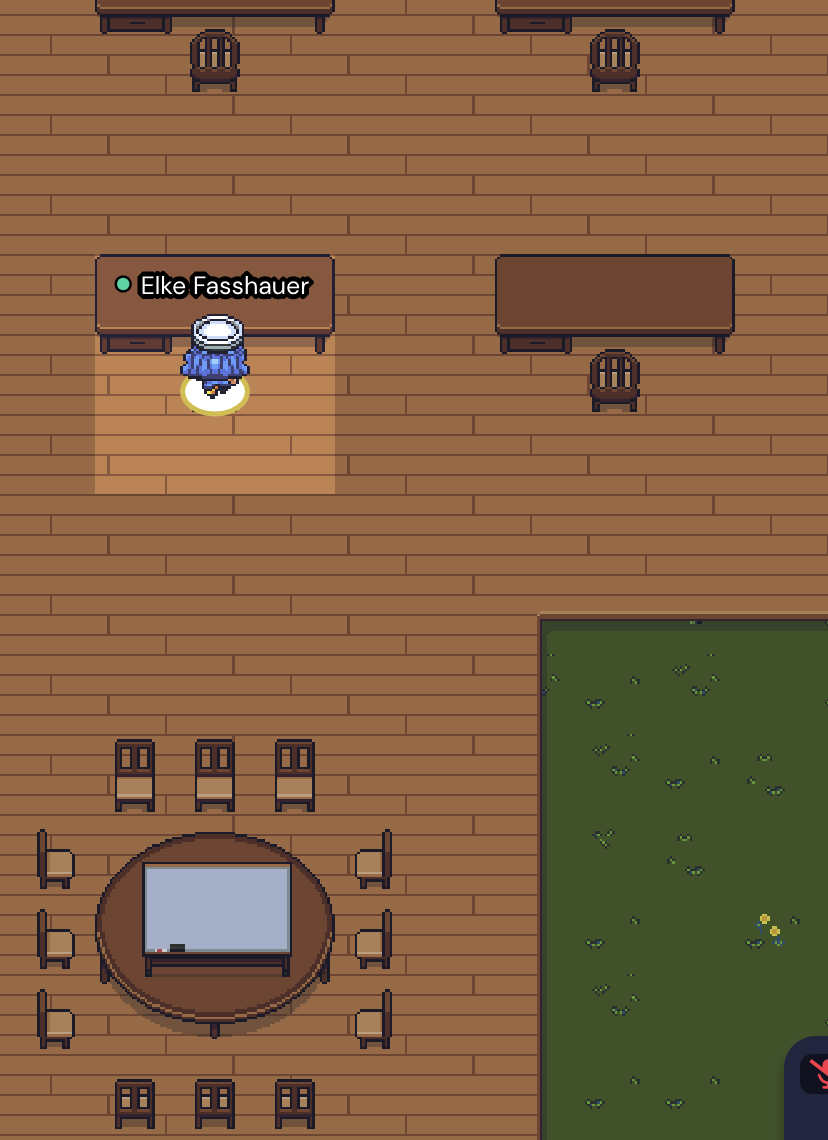
\includegraphics[width=0.45\textwidth]{pics/navigation/sit_small_desk_2.png}
\hfill
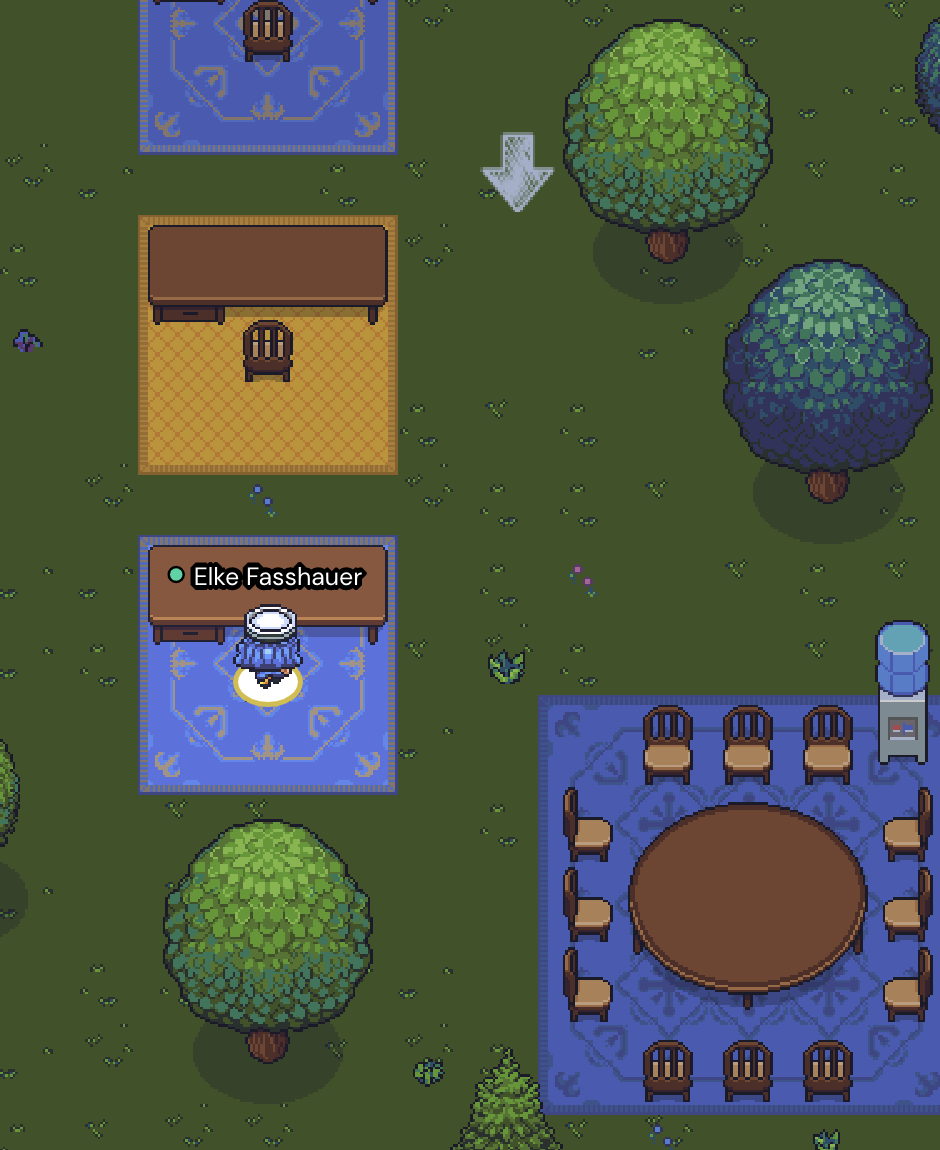
\includegraphics[width=0.45\textwidth]{pics/navigation/sit_small_desk_1.png}
\end{center}

\end{frame}


\begin{frame}{Motivation}

\begin{center}
  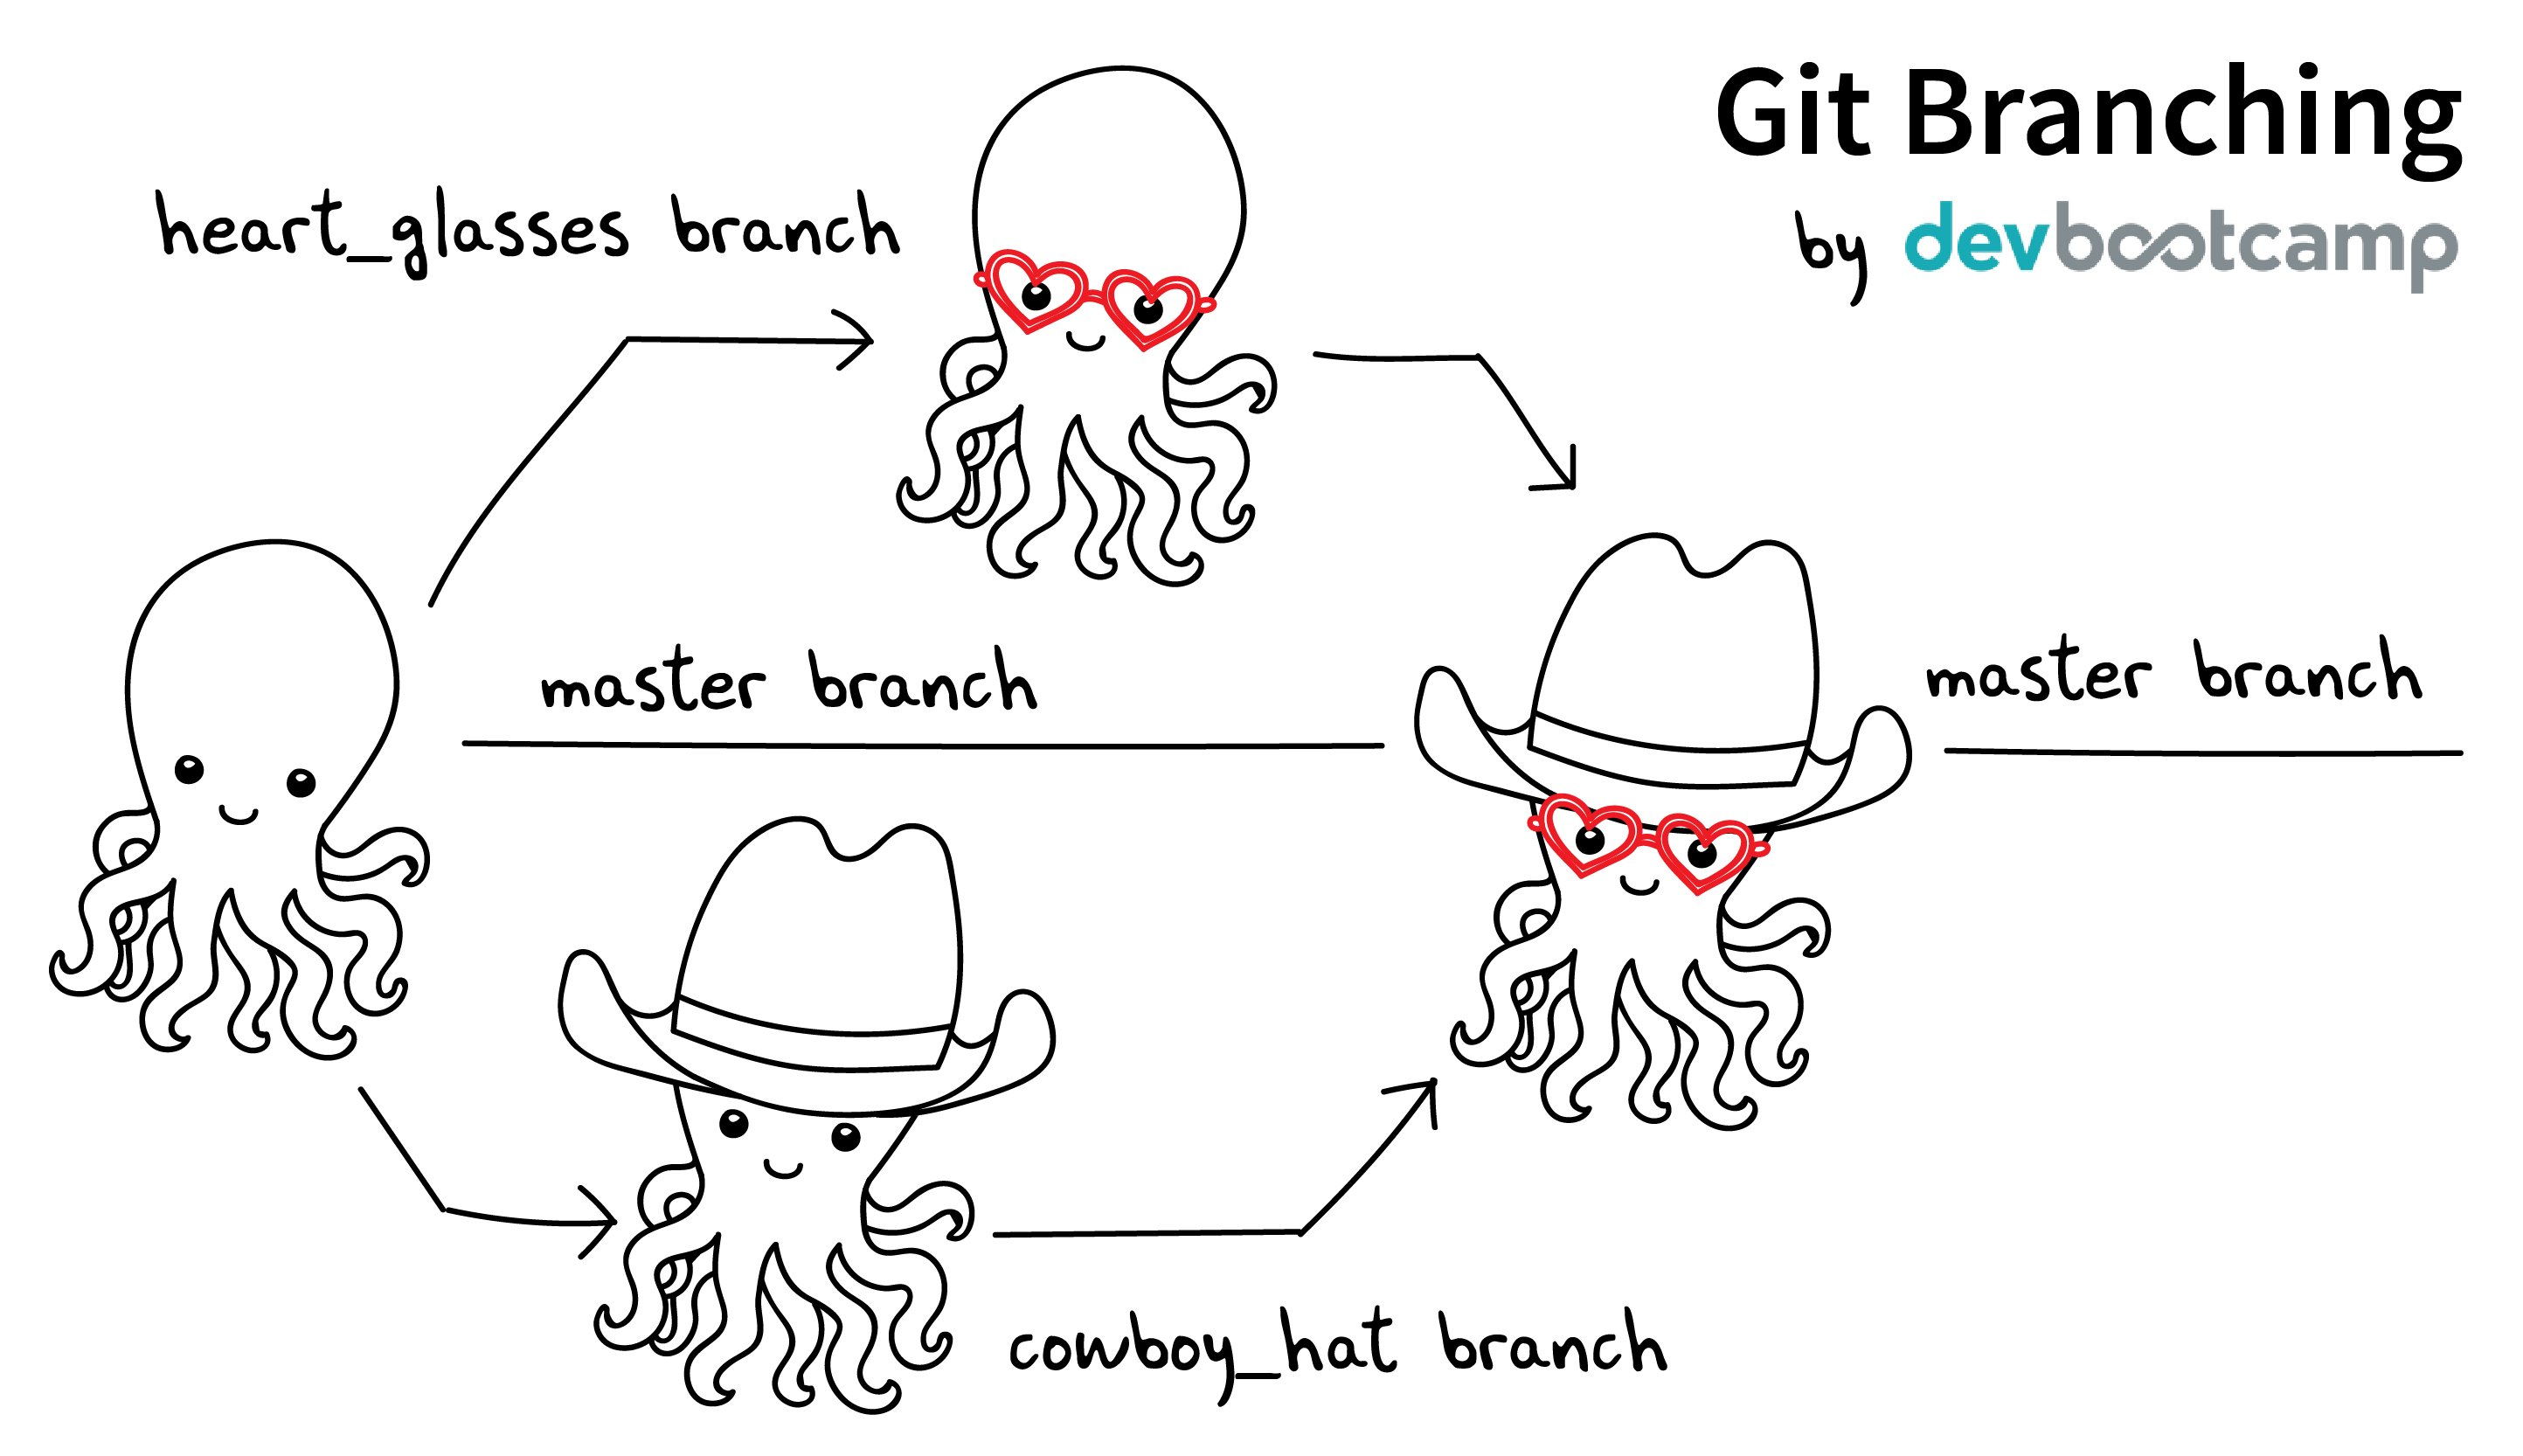
\includegraphics[width=0.8\textwidth]{../01_basics/pics/merging_pic.jpg}
\end{center}


%\begin{semiverbatim}
%git status
%\end{semiverbatim}

\tiny
\begin{tabular}{l}
Coderefinery: \url{https://twitter.com/jay_gee/status/703360688618536960}
\end{tabular}

\end{frame}

%\begin{frame}{Merging}

Exercises:

\begin{itemize}
 \item On which branch are we?
 \item Creating and working with branches
 \item Exercise: create and commit to branches
 \item Merging branches
 \item Deleting branches safely
 \item Summary
 \item Typical workflow
\end{itemize}

\end{frame}

\begin{frame}{Workflow: Where are we?}
\footnotesize

\onslide<2->{
\begin{block}{}
\begin{semiverbatim}
\$ git branch


\only<3->{
* \textcolor{green}{main}
}
\end{semiverbatim}
\end{block}
}

\onslide<4->{
\begin{block}{What our file looks like}
\begin{semiverbatim}
Test


firrst line


\end{semiverbatim}
\end{block}
}

\end{frame}

\begin{frame}{Workflow: Creating branches}
\footnotesize

\onslide<2->{
\begin{block}{Let's do some more work}
\begin{semiverbatim}
\$ git branch new\_content main

\onslide<3->{
\$ git checkout new\_content
}

\onslide<4->{
\$ git branch new\_content main
}


\only<5->{
main

* \textcolor{green}{new\_content}
}
\end{semiverbatim}
\end{block}
}

\onslide<6->{
\begin{block}{What our file looks like}
\begin{semiverbatim}
Test


firrst line


second line


\end{semiverbatim}
\end{block}
}

\end{frame}

\begin{frame}{Workflow: Working with multiple branches}
\footnotesize

\onslide<2->{
\begin{block}{Correct typo}
\begin{semiverbatim}
\$ git checkout main

\onslide<3->{
\$ git branch typo main
}

\onslide<4->{
\$ git checkout typo
}

\onslide<5->{
\$ git branch
}

\only<6->{
main

new\_content

* \textcolor{green}{typo}

}
\end{semiverbatim}
\end{block}
}

\only<7->{
\begin{block}{What our file looks like}
\begin{semiverbatim}
Test


firrst line


\end{semiverbatim}
\end{block}
}

\end{frame}

\begin{frame}{Workflow: Merging branches}
\footnotesize

\onslide<2->{
\begin{block}{}
\begin{semiverbatim}
\$ git merge main

\onslide<3->{
\$ git checkout main
}

\onslide<4->{
\$ git merge typo
}

\onslide<5->{
\$ git branch -d typo
}

\onslide<6->{
\$ git branch
}



\only<7->{
* \textcolor{green}{main}

new\_content
}
\end{semiverbatim}
\end{block}
}

\onslide<8->{
\begin{block}{What our file looks like}
\begin{semiverbatim}
Test


first line


\end{semiverbatim}
\end{block}
}

\end{frame}

\begin{frame}{Workflow: Merging branches}
\footnotesize

\onslide<2->{
\begin{block}{}
\begin{semiverbatim}
\$ git checkout new\_content

\onslide<3->{
\$ git merge main
}

\onslide<4->{
\$ git checkout main
}

\onslide<5->{
\$ git merge new\_content
}




\end{semiverbatim}
\end{block}
}

\onslide<6->{
\begin{block}{What our file looks like}
\begin{semiverbatim}
Test


first line


second line


\end{semiverbatim}
\end{block}
}

\end{frame}

\begin{frame}{Motivation}

\begin{center}
  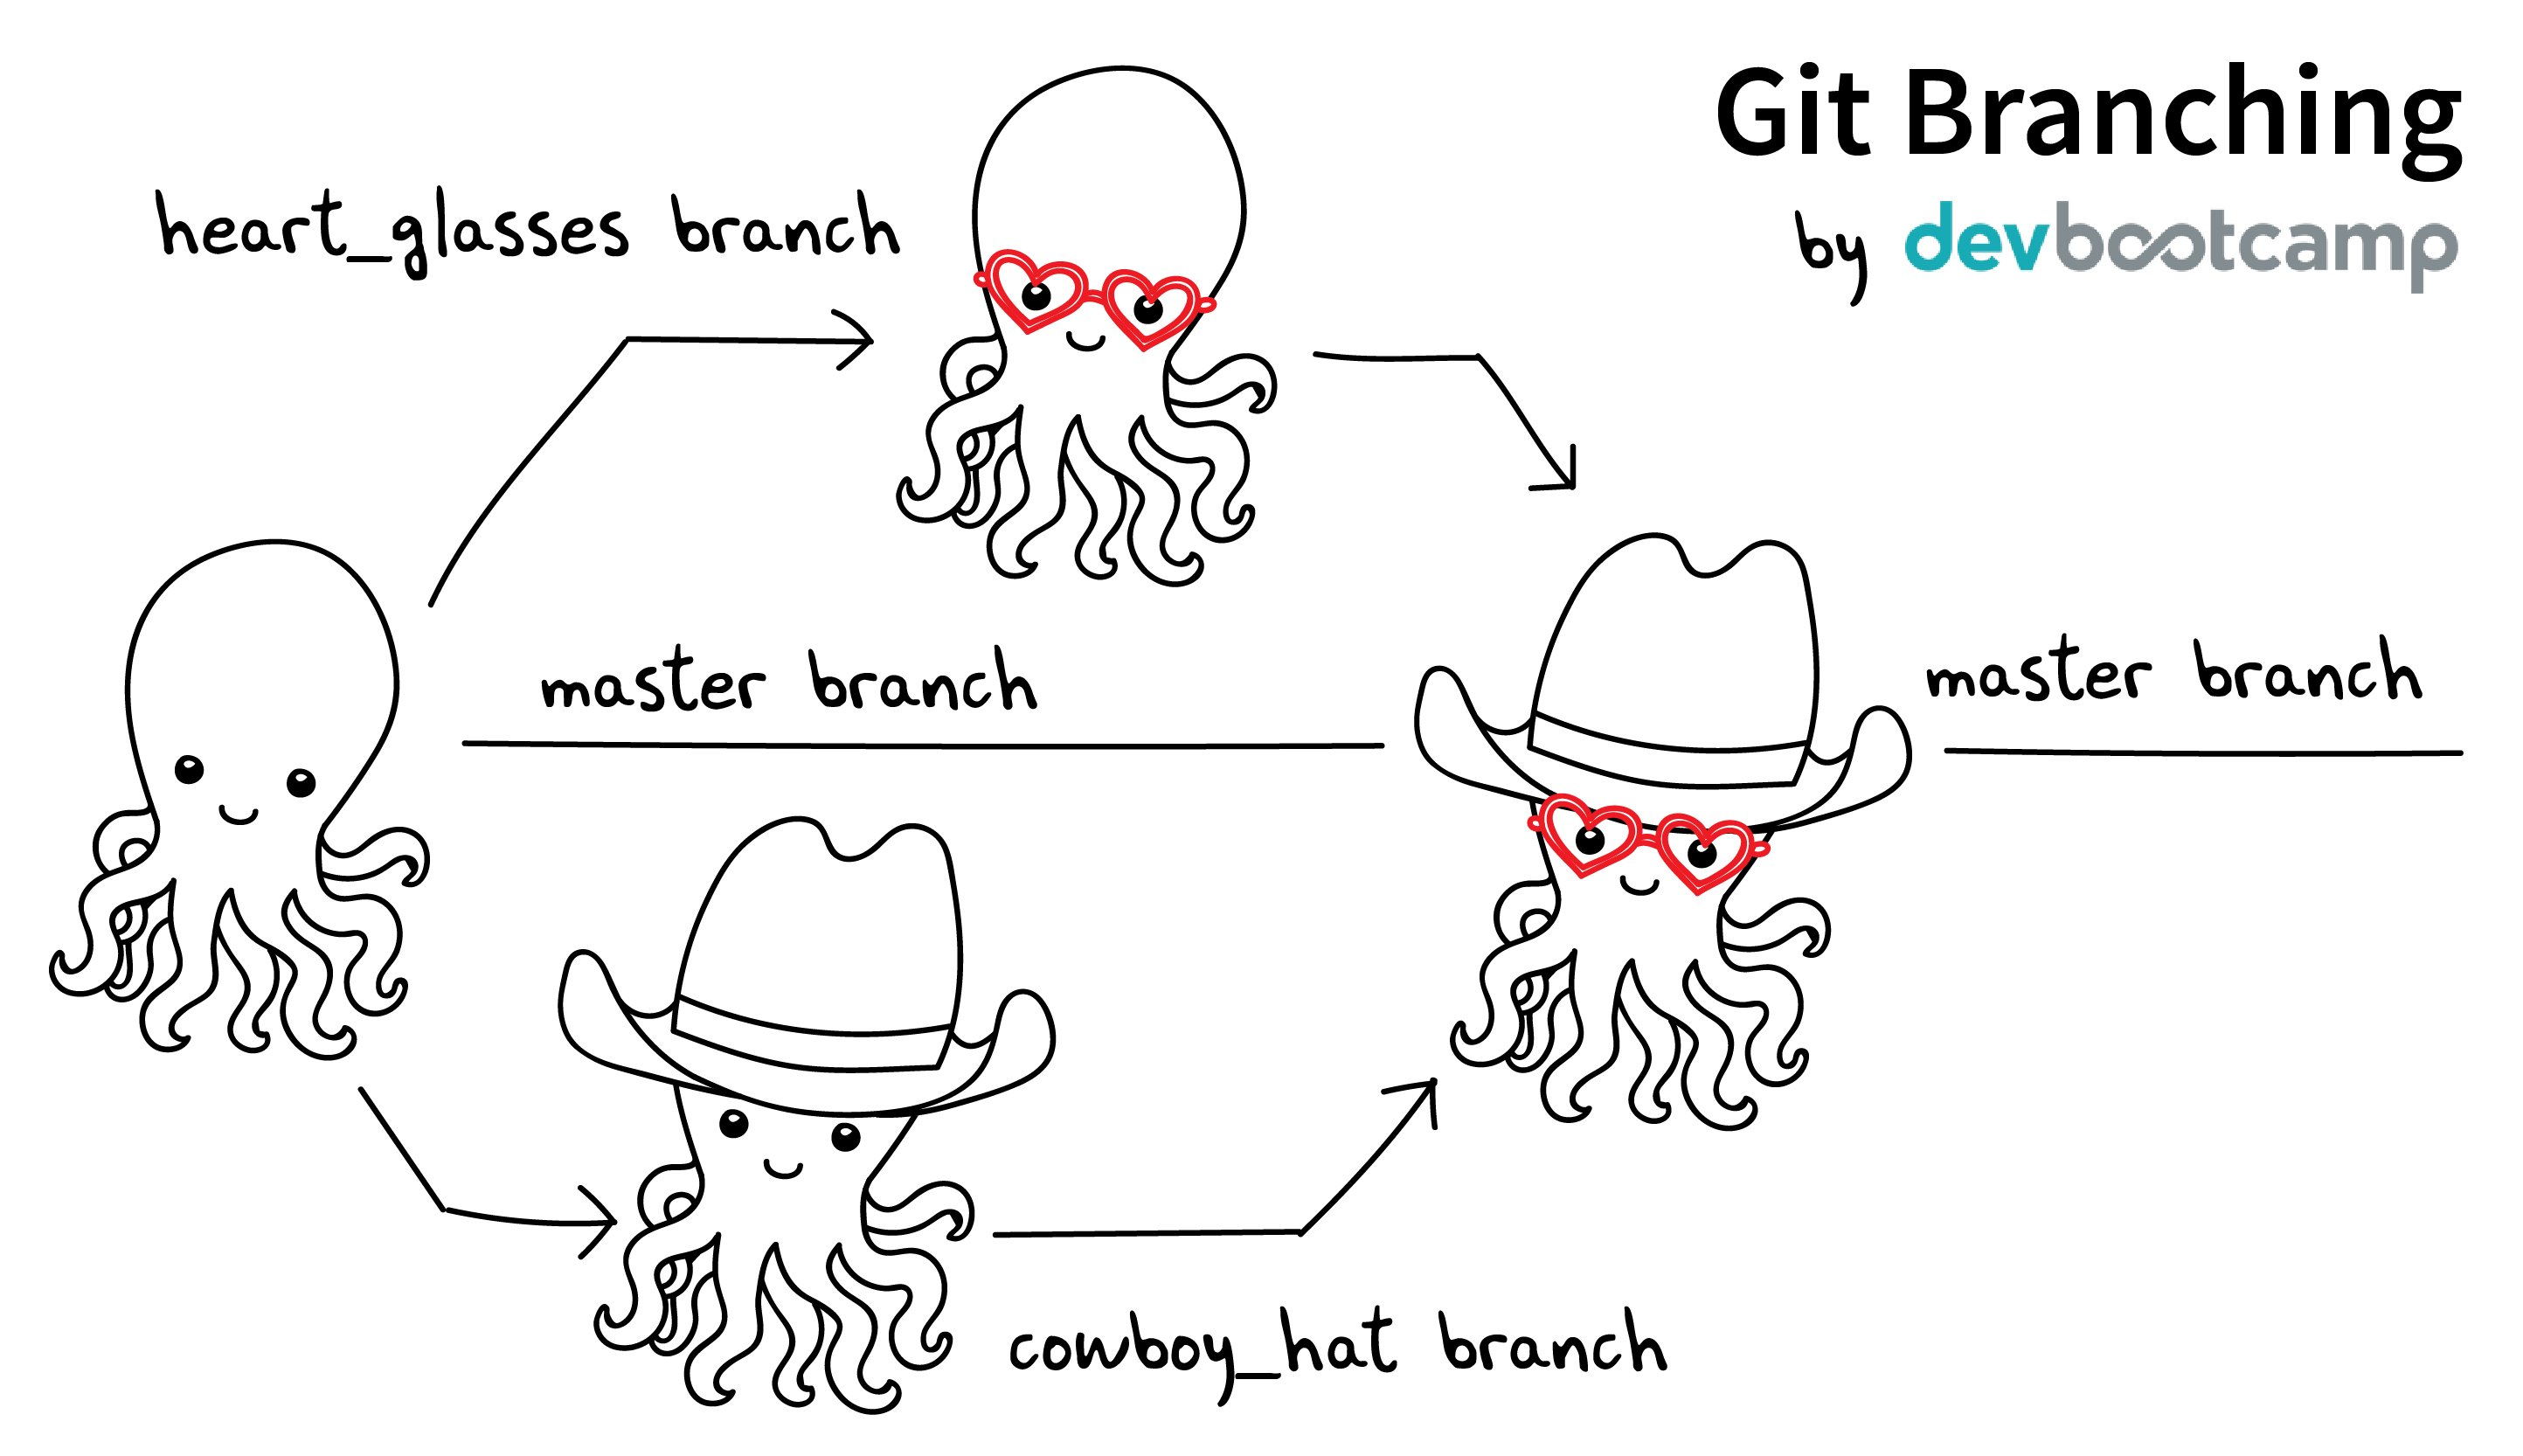
\includegraphics[width=0.8\textwidth]{../01_basics/pics/merging_pic.jpg}
\end{center}


%\begin{semiverbatim}
%git status
%\end{semiverbatim}

\tiny
\begin{tabular}{l}
Coderefinery: \url{https://twitter.com/jay_gee/status/703360688618536960}
\end{tabular}

\end{frame}


%\begin{frame}{Where to go for the exercise}

\begin{center}
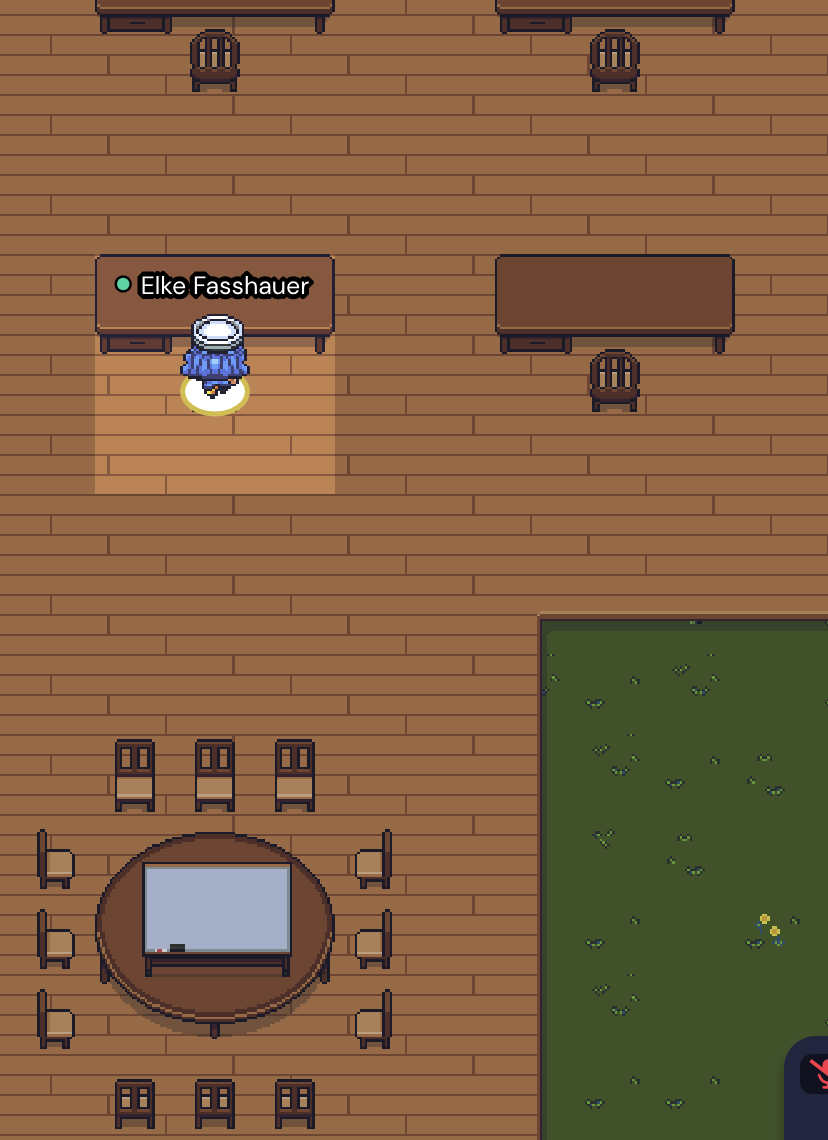
\includegraphics[width=0.45\textwidth]{pics/navigation/sit_small_desk_2.png}
\hfill
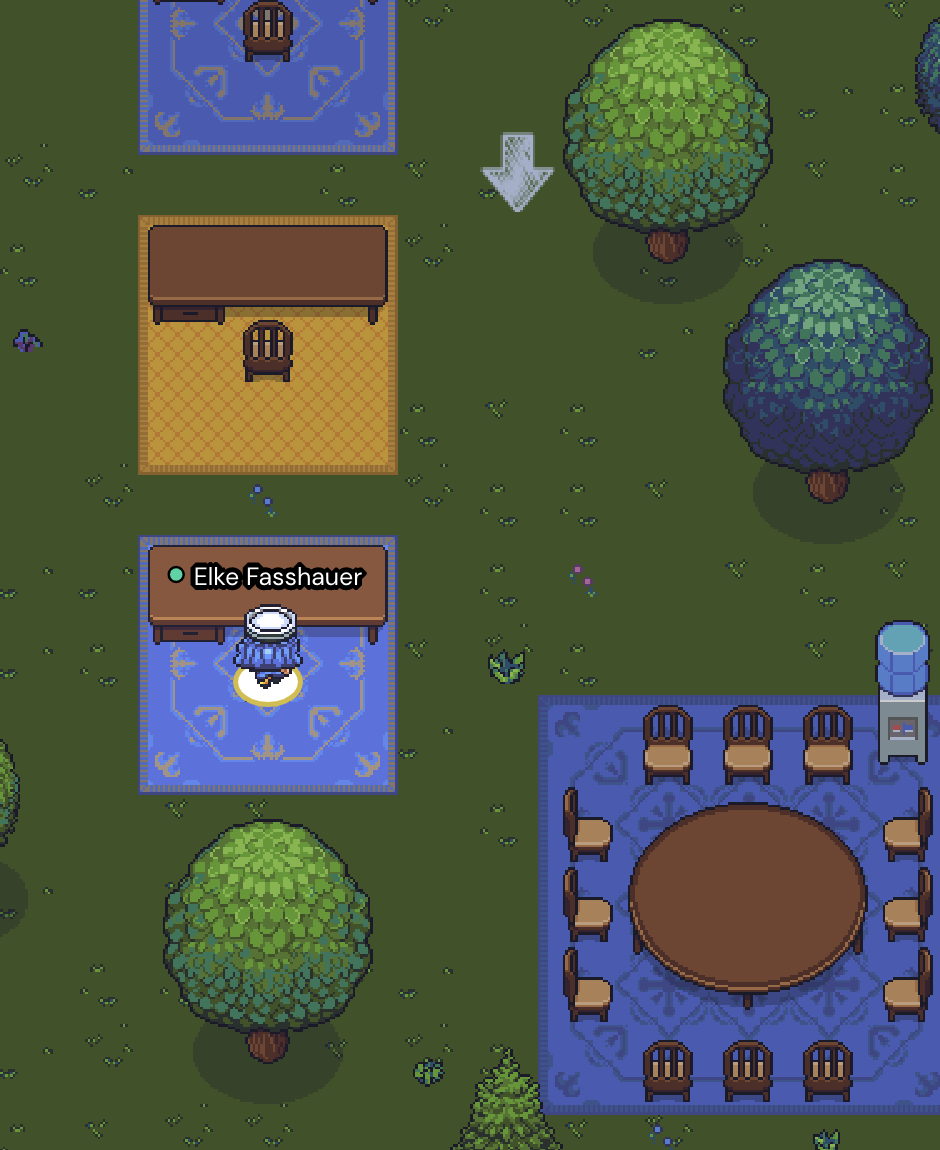
\includegraphics[width=0.45\textwidth]{pics/navigation/sit_small_desk_1.png}
\end{center}

\end{frame}



\end{document}
